\documentclass[tikz,border=5pt]{standalone}

\usepackage[T1]{fontenc}
\usepackage{lmodern}
\usepackage{amsmath}
\usetikzlibrary{arrows.meta,calc,decorations.pathreplacing,shapes.geometric}

\definecolor{positivebranch}{RGB}{0,114,178}
\definecolor{negativebranch}{RGB}{213,94,0}
\definecolor{targetgrey}{RGB}{85,85,85}

\begin{document}
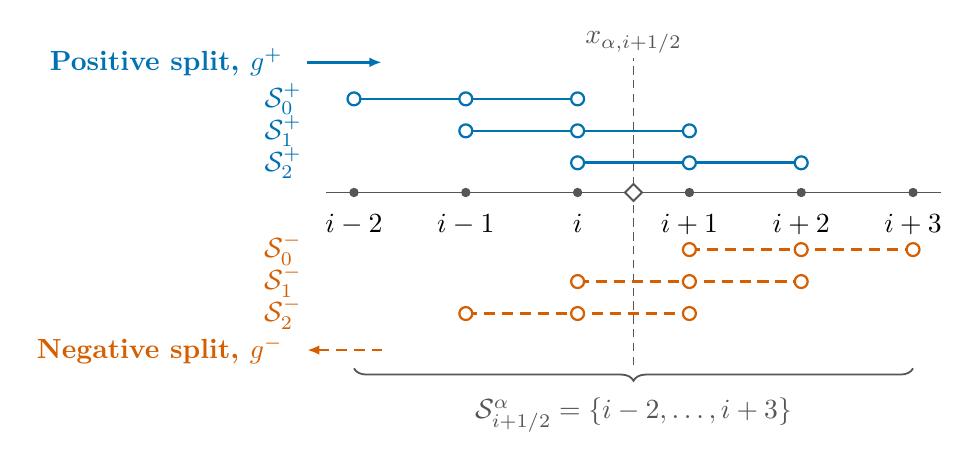
\begin{tikzpicture}[
    x=1.42cm,
    y=0.58cm,
    >=Latex,
    stencil plus/.style={
      positivebranch,
      line width=0.95pt
    },
    stencil minus/.style={
      negativebranch,
      line width=0.95pt,
      dash pattern=on 4pt off 2.5pt
    },
    stencil node plus/.style={
      circle,
      draw=positivebranch,
      fill=white,
      line width=0.8pt,
      inner sep=1.65pt
    },
    stencil node minus/.style={
      circle,
      draw=negativebranch,
      fill=white,
      line width=0.8pt,
      inner sep=1.65pt
    }
]

% Coordinate labels and target location.
\foreach \x/\lab in {
  0/{i-2},
  1/{i-1},
  2/{i},
  3/{i+1},
  4/{i+2},
  5/{i+3}
}{
  \coordinate (c\x) at (\x,0);
  \fill[targetgrey] (c\x) circle (1.7pt);
  \node[below=4.5pt] at (c\x) {$\lab$};
}

\draw[targetgrey,line width=0.65pt] (-0.25,0) -- (5.25,0);
\draw[targetgrey,densely dashed,line width=0.7pt]
  (2.5,-3.78) -- (2.5,3.15);
\node[
  fill=white,
  inner xsep=2.5pt,
  inner ysep=1.5pt,
  text=targetgrey
] at (2.5,3.28) {$x_{\alpha,i+1/2}$};
\node[
  draw=targetgrey,
  fill=white,
  diamond,
  inner sep=1.6pt,
  line width=0.7pt
] at (2.5,0) {};

% Positive characteristic branch.
\node[
  anchor=east,
  text=positivebranch,
  font=\bfseries
] at (-0.55,2.85) {Positive split, \(g^{+}\)};
\draw[stencil plus,-{Latex[length=4.5pt,width=3.5pt]}]
  (-0.42,2.85) -- (0.25,2.85);

\node[anchor=east,text=positivebranch] at (-0.38,2.05)
  {$\mathcal{S}^{+}_{0}$};
\draw[stencil plus] (c0 |- 0,2.05) -- (c2 |- 0,2.05);
\foreach \x in {0,1,2}
  \node[stencil node plus] at (c\x |- 0,2.05) {};

\node[anchor=east,text=positivebranch] at (-0.38,1.35)
  {$\mathcal{S}^{+}_{1}$};
\draw[stencil plus] (c1 |- 0,1.35) -- (c3 |- 0,1.35);
\foreach \x in {1,2,3}
  \node[stencil node plus] at (c\x |- 0,1.35) {};

\node[anchor=east,text=positivebranch] at (-0.38,0.65)
  {$\mathcal{S}^{+}_{2}$};
\draw[stencil plus] (c2 |- 0,0.65) -- (c4 |- 0,0.65);
\foreach \x in {2,3,4}
  \node[stencil node plus] at (c\x |- 0,0.65) {};

% Negative characteristic branch. The stencil order mirrors the positive branch.
\node[anchor=east,text=negativebranch] at (-0.38,-1.25)
  {$\mathcal{S}^{-}_{0}$};
\draw[stencil minus] (c3 |- 0,-1.25) -- (c5 |- 0,-1.25);
\foreach \x in {3,4,5}
  \node[stencil node minus] at (c\x |- 0,-1.25) {};

\node[anchor=east,text=negativebranch] at (-0.38,-1.95)
  {$\mathcal{S}^{-}_{1}$};
\draw[stencil minus] (c2 |- 0,-1.95) -- (c4 |- 0,-1.95);
\foreach \x in {2,3,4}
  \node[stencil node minus] at (c\x |- 0,-1.95) {};

\node[anchor=east,text=negativebranch] at (-0.38,-2.65)
  {$\mathcal{S}^{-}_{2}$};
\draw[stencil minus] (c1 |- 0,-2.65) -- (c3 |- 0,-2.65);
\foreach \x in {1,2,3}
  \node[stencil node minus] at (c\x |- 0,-2.65) {};

\node[
  anchor=east,
  text=negativebranch,
  font=\bfseries
] at (-0.55,-3.45) {Negative split, \(g^{-}\)};
\draw[stencil minus,{Latex[length=4.5pt,width=3.5pt]}-]
  (-0.42,-3.45) -- (0.25,-3.45);

% Union of the two mirrored five-point reconstructions.
\draw[
  decorate,
  decoration={brace,mirror,amplitude=4.5pt},
  targetgrey,
  line width=0.65pt
] (0,-3.85) -- (5,-3.85);
\node[below=7pt,text=targetgrey] at (2.5,-3.85)
  {$\mathcal{S}_{i+1/2}^{\alpha}=\{i-2,\ldots,i+3\}$};

\end{tikzpicture}
\end{document}
